
\documentclass[\PRJWD/Thick_TQFTs_and_Quantum_Information.tex]{subfiles}

\begin{document}

\section{Parallel Field Theory}

In definition \ref{defn:sing_man_tqft}, we associated to each object a tensor
power of some algebra $A$; to each vertical $1$--morphism, the identity on $A$;
to each horizontal $1$--morphism, a linear map from a tensor power of $A$ to
another; to each $2$--morphism, a smooth family of linear maps. This data
suggests a codomain double category of our single manifold TQFT, which we define
next.

\subsection{Double Category of Finite Dimensional Vector Spaces}

We consider as the object or $0$--morphism category of the codomain double
category the monoidal category of finite-dimensional, real (or complex) vector
spaces $\FVect_{\K}$ for $\K = \R$ or $\C$. We then notice a categorification
of the collection of morphisms of this category as follows.

We consider the collection of all morphisms of $\FVect_{\K}$,
\[
  \s{L} := \set[f]{f \in \Hom_{\FVect_{\K}}(U, V), U, V \in \Ob \FVect_{\K}}
\]
as the object collection of the horizontal $1$--morphism category of our double
category. For each such map, we choose some $p \times q$ matrix representation
$[a_{ij}]$ which yields a mapping $\iota : \s{L} \to \M_{N}(\C)$, where
$\M_{\N}(\C)$ is the set of infinite complex matrices indexed by $\N \times \N$,
defined by:
\[
  \iota(a)_{ij} = \begin{cases}
    a_{ij} & 1 \leq i \leq p, 1 \leq j \leq q \\
    0      & \text{otherwise}
  \end{cases}
\]

This provides a notion of $2$--morphism for our double category under
construction. We notice that the Banach space $\s{B}$ of bounded operators on
the Hilbert space space $\ell^2(\N)$ can be seen as a subset of $\M_{\N}$, such
that $\s{L} \subset \s{B} \subset \M_{\N}$. It is well-known that $\s{B}$, being
a Banach space, is a simply-connected topological space. Now, for $a$ and $a'$
in $\s{L}$, we define a $2$--morphism to be a homomotpy class of paths $\alpha$
from $\iota(a)$ to $\iota(')$ in $\s{B}$, which we denote as
$\alpha : a \To a'$. By the fact the fundamental groupoid
$\Pi_1(\s{B})$ is a category, our $2$--morphisms have a strictly associative and
unital composition.  We note that the fundamental groupoid $\Pi_1(\s{B})$ is not
our morphism category -- it only supplies morphisms for $\s{L}$. An instance of
why the distinction is important is that a single morphism in $\Pi_1(\s{B})$
might represent morphisms between two different pairs of objects in $\s{L}$,
depending on the chosen matrix representations.

It is worthwhile observing the action of composition and tensor products of
linear maps on $2$--morphisms. We first notice that iota can be defined so that
it is multiplicative in two ways:
\[
  \iota(b \circ a) := \iota(b) \cdot \iota(a)
\]
where the right-hand-side product is the matrix product in $\M_{\N}(\C)$, and
\[
  \iota(a \tensor b) := \iota(a) \tensor \iota(b)
\]
where the $\tensor$ on the right is given by the Kronecker product. Now,
consider pairs of homotopic paths
$\alpha_1, \alpha_2 : a \To a'$ and
$\beta_1, \beta_2 : b \To b'$, where $b, a$ and $b', a'$ are
composeable pairs of linear maps. We consider the pointwise composites:
\begin{equation}\label{eqn:pointwise_comp}
  (\beta_i \circ \alpha_i)(t) := \beta_i(t) \circ \alpha_i(t), t \in [0, 1],
    i \in \set{1, 2}
\end{equation}
Now, the $\beta_i \circ \alpha_i$ are clearly paths
$b \circ a \To b' \circ a'$ in $\s{B}$-- we wish to show that
they are homotopic, making the operation well-defined on homomotopy classes of
paths. It suffices to observe that $\s{B}$ is simply connected, so that there is
exactly one class of homotopic paths between two points in $\Pi_1(\s{B})$.

Consider again elements
$a : U \to V, a' : U' \to V', b : X \to Y, b' : X' \to Y'$ of $\s{L}$. We define
\[
  n_x := \dim \dom x, m_x := \dim \codom x, x \in \set{a, a', b, b'}
\]
and
\[
  N_{x} = N_{x'} := \max\set{n_x, n_{x'}},
  M_{x} = M_{x'} := \max\set{m_x, m_{x'}}, x \in \set{a, b}
\]
We then have matrix representations of each $x \in \set{a, a', b, b'}$:
\[
  \iota'(x) := [\iota(x)_{ij}] \in \M_{M_x \times N_x}(\C)
\]
Now, $\M_{M_x \times N_x}(\C)$, being simply connected, has a path
$\gamma_x$ from $\iota'(x)$ to $\iota'(x')$ for each $x \in \set{a, b}$. In
fact, using the inclusion $\M_{M_x \times N_x}(\C) \hto \s{B}$ induced by
$\iota$, each $\gamma_x$ yields a path $\wh{\gamma_x}$ in $\s{B}$ from
$\iota(x)$ to $\iota(x')$, with its image contained in $\s{L}$. Since $\s{B}$ is
simply connected, every path in $\s{B}$ from $\iota(x)$ to $\iota(x')$ is
homotopic to $\wh{\gamma_x}$. Furthermore,
$\wh{\gamma_a}(t) \tensor \wh{\gamma_b}(t)$ is also a path from
$\iota(a \tensor a') = \iota(a) \tensor \iota(a')$ to
$\iota(b \tensor b') = \iota(b) \tensor \iota(b')$ in $\s{B}$, to which all
other paths with the same endpoints are homotopic. This shows that
\[
  (\wh{\gamma_a} \tensor \wh{\gamma_b})(t) :=
    \wh{\gamma_a}(t) \tensor \wh{\gamma_b}(t)
\]
is well-defined on homotopy classes of paths in $\Pi_1(\s{B})$. For
associativity of $\tensor$, we observe that
\[
  \iota(a \tensor (b \tensor c))
    = \iota(a) \tensor \iota(b) \tensor \iota(c)
    = \iota((a \tensor b) \tensor c)
\]
so that the constant path on $\iota(a) \tensor \iota(b) \tensor \iota(c)$
functions as the associator
\[
  a \tensor (b \tensor c) \to (a \tensor b) \tensor c
\]
For unitality of $\tensor$, we take the matrix $1_{\tensor} \in \s{B}$ whose
$(i, j)$ entry is $1$ if $i = j = 1$ and is $0$ otherwise, and then we observe:
\[
  \iota(a \tensor \id_{\K}) = \iota(a) \tensor 1_{\tensor} = \iota(a)
    = \iota(\id_{\K} \tensor a)
\]
so that the constant path on $\iota(a)$ functions as a left and right unitor.

We then take horizontal composition to be given by composition of linear maps
which is strictly associative and unital, with coherence following from that in
the category of vector spaces. The source and target functors are obvious -- we
send each linear map to its domain and codomain respectively. The unit functor
is also obvisous -- we send each object to its identity linear map.
The axioms of a monoidal double category given in the unpacked version of
definition 2.9 in \cite[5]{SymMonBicat} are also easily verified.

\TODO{Add an appendix entry for this verification.}

We compile these results into the following definition:
\begin{defn}[Double Category of Finite Dimensional Vector Spaces]
The following data form a monoidal double category:
\begin{enmrt}
\li Object category: $\FVect_{\K}$
\li Morphism category: $\s{L}$
\li Source functor: $\dom : (f : X \to Y) \mapsto X$
\li Target functor: $\codom : (f : X \to Y) \mapsto Y$
\li Unit functor: $V \mapsto \id_V$
\li Horizontal composition: $(g, f) \mapsto g \circ f$
\li Horizontal composition associator: constant path on
$\iota(a \circ b \circ c)$
\li Horizontal composition unitor: constant path on $\iota(\id_V)$, for a vector
space $V$
\li Monoidal product: $\tensor$ in appropriate contexts defined above
\li Monoidal unit: $\K$ for the object category and $\id_{\K}$ for the morphism
category
\li Monoidal associators: constant path on
$\iota(a) \tensor \iota(b) \tensor \iota(c)$ as an associator
\[
  a \tensor (b \tensor c) \to (a \tensor b) \tensor c
\]
\li Monoidal unitor: constant path on $\iota(\id_{\K}) = 1_{\tensor}$
\end{enmrt}
This is called the monoidal double category of finite dimensional $\K$--vector
spaces and is denoted $\FFVect_{\K}$.
\end{defn}

We finally note that if the choice of matrix representations poses foundational
problems, we can easily switch to the skeleton of $\FVect_{\K}$ consisting of
the spaces $\K^n$ for all $n \in \N$.

%\begin{enmrt}
%
%\li The object category is easily seen to be a monoidal category -- it is the
%monoidal category generated by a single object $A$ in a monoidal category (of
%vector spaces) and associators and unitors between its monoidal products.
%
%The morphism category consists of linear maps of the form:
%\[
%  a : A^{\tensor n} \to A^{\tensor m} \text{ and }
%  b : A^{\tensor n'} \to A^{\tensor m'}
%\]
%with some parenthesizing pattern for each domain or codomain tensor power. The
%tensor product $a \tensor b$ gives the object function of the monoidal product
%functor. The pointwise tensor product \ref{eqn:pointwise_tensor} is the morphism
%function of the monoidal product functor.
%
%\li The monoidal unit of the object category is the base field, say $\C$, and
%the unit horizontal $1$--morphism is also the monoidal unit for horizontal
%$1$--morphisms:
%\[
%  a \tensor 1_{\C} = a = 1_{\C} \tensor a
%\]
%\end{enmrt}

\subsection{Thick Tangles and Transport Graphs}

Having established a codomain double category, we look towards extending our
notion of TQFTs based on transport graphs in a single manifold to transport
graphs in cobordisms equipped with connections. For simplicity, we only consider
thick tangles equipped with connections, at the moment. Recall that a thick
tangle $X \to Y$ is a smooth surfaces $M$ with boundary $W_0 \amalg W_1$ with
equipped with smooth maps $a_M : X \to M, b_M : Y \to M$ such that $a_M$ and
$b_M$ are diffeomorphisms onto $W_0$ and $W_1$ respectively, and an embedding
$d_M : M \to \R \times [0, 1]$ (satisfying some additional properties, which we
will not need at the moment).

We consider the generating thick tangles equipped with transport graphs.
The following examples of transport graphs in the pair-of-pants, cap and their
duals gives us an idea of the structures we are dealing with:
\[
% Pants:
\begin{tikzpicture}[scale=0.55]
\pants{0, 0}
\lblvert{0, -4}{pants}{\footnotesize pair-of-pants}
\colvert{blue}{-2, 6}{a1}
\lblvert{-2.85, 6}{a1l}{\footnotesize $a_1$}
\colvert{blue}{-2, 4}{a2}
\lblvert{-2.85, 4}{a2l}{\footnotesize $a_2$}
\colvert{blue}{2, 5}{a3}
\lblvert{2.85, 5}{a3l}{\footnotesize $a_3$}
\midarrow{a1}{a3}
\midarrow{a2}{a3}
% Path 1 --> 3
\colvert{blue}{-1.55, 1.65}{a1p}
\lblvert{-1.55, 2.1}{a1pl}{\footnotesize $a_1$}
\colvert{blue}{1.5, -0.75}{a3p1}
\lblvert{1.5, -0.3}{a3p1l}{\footnotesize $a_3$}
\midarrowc{a1p}{0, 1}{0, -1}{a3p1};
% Path 2 --> 3
\colvert{blue}{-1.25, -1.95}{a2p}
\lblvert{-1.25, -1.45}{a2pl}{\footnotesize $a_2$}
\colvert{blue}{1.25, 0.35}{a3p2}
\lblvert{1.25, 0.75}{a3p2l}{\footnotesize $a_3$}
\midarrowc[0.35]{a2p}{0, -2}{1, 0.25}{a3p2}
\end{tikzpicture}
\qquad
% Cap:
\begin{tikzpicture}[scale=0.55]
\capcob{0, 0}
\lblvert{-1.5, -4}{caplbl}{\footnotesize cap}
\colvert{blue}{-2, 5}{a1}
\colvert{green!55!black}{-1, 5}{a2}
\midarrow{a1}{a2}
% Path 1 --> 2
\colvert{blue}{-1.75, 0.75}{a1p}
\colvert{green!55!black}{-1.35, -0.45}{a2p}
\midarrowc{a1p}{-1.75, -0.05}{-1, 0}{a2p}
\end{tikzpicture}
\qquad
% Cup:
\begin{tikzpicture}[scale=0.55]
\cupcob{0, 0}
\lblvert{1.5, -4}{caplbl}{\footnotesize cup}
\colvert{green!55!black}{1, 5}{a1}
\colvert{blue}{2, 5}{a2}
\midarrow{a1}{a2}
% Path 1 --> 2
\colvert{green!55!black}{1.75, 0.75}{a1p}
\colvert{blue}{1.75, -0.75}{a2p}
\midarrowc{a1p}{1.1, 0}{1.1, 0}{a2p}
\end{tikzpicture}
\qquad
% Copants
\begin{tikzpicture}[scale=0.55]
\copants{0, 0}
\lblvert{0, -4}{copants}{\footnotesize co-pair-of-pants}
\colvert{blue}{2, 6}{a1}
\lblvert{2.85, 6}{a1l}{\footnotesize $a_1$}
\colvert{blue}{2, 4}{a2}
\lblvert{2.85, 4}{a2l}{\footnotesize $a_2$}
\colvert{blue}{-2, 5}{a3}
\lblvert{-2.85, 5}{a3l}{\footnotesize $a_3$}
\midarrow{a3}{a1}
\midarrow{a3}{a2}
% Path 3 --> 1
\colvert{blue}{-1.25, 0}{a3p}
\lblvert{-1.25, 0.45}{a3pl}{\footnotesize $a_3$}
\colvert{blue}{1.5, 1.75}{a1p}
\lblvert{1.5, 2.25}{a1pl}{\footnotesize $a_1$}
\midarrowc{a3p}{0, 0}{-0.5, 1}{a1p}
% Path 3 --> 2
\colvert{blue}{1.5, -1.75}{a2p}
\lblvert{1.5, -2.25}{a2pl}{\footnotesize $a_2$}
\midarrowc{a3p}{0, 0}{-0.5, -1}{a2p}
\end{tikzpicture}
\]
We recall that edges that share an end-point need not map to paths that share an
end-point, as we see in the left diagram. At the same time, paths are allowed to
intersect. We also note that we have chosen the pretransport graphs so as to
match their sources and targets with the sources and targets of their realizing
cobordisms. We now turn our attention to the cylinder. We observe that the
cylinder is a cobordism $I \to I$. On the transport graph side, morphisms from a
single blue vertex to another can be any path with blue end-points including the
path consisting of a single blue vertex. However, the gluing unit for the single
blue vertex, on either side, is the single blue vertex itself. Hence, we will
consider the following transport graphs in the cylinder:
\[
\begin{tikzpicture}[scale=0.55]
\idcob{0, 0}
\colvert{blue}{0, 2}{a}
\lblvert{0, -2}{lbl}{\footnotesize cylinder without paths}
\end{tikzpicture}
\qquad \qquad
\begin{tikzpicture}[scale=0.55]
\idcob{0, 0}
\lblvert{0, -2}{lbl}{\footnotesize cylinder with paths}
\colvert{blue}{-2, 2}{a1}
\colvert{blue}{2, 2}{a2}
\midarrow{a1}{a2}
\colvert{blue}{-1.5, -0.15}{a1p}
\colvert{blue}{1.5, 0.15}{a2p}
\midarrowc{a1p}{0, 0.45}{0, -0.45}{a2p}
\end{tikzpicture}
\]

\begin{exm}
We take the example from our first description of the double categorical
approach and adapt it to this setting. The following is one possible diagram:
\[\begin{tikzpicture}[scale=0.33]

\idcobup{1, 0}
\colvert{blue}{-0.5, -1.85}{s}
\colvert{blue}{2, 0.25}{t}
\midarrowc{s}{0, -2}{2, -1}{t}

\coordinate (cntr) at (1, 4);
\pants{cntr}
\colvert{blue}{$(cntr) + (-1.5, 2)$}{s1}
\colvert{blue}{$(cntr) + (-1.5, -2)$}{s2}
\colvert{blue}{$(cntr) + (1.25, 0)$}{t}
\midarrowc{s1}{$(cntr) + (0, 2)$}{$(cntr) + (0, 0)$}{t}
\midarrowc{s2}{$(cntr) + (0, 1)$}{$(cntr) + (0, -1)$}{t}

\coordinate (cntr) at (5, 2);
\pants{cntr}
\colvert{blue}{$(cntr) + (-1.5, 2)$}{s1}
\colvert{blue}{$(cntr) + (-1.5, -2)$}{s2}
\colvert{blue}{$(cntr) + (1.25, 0)$}{t}
\midarrowc{s1}{$(cntr) + (0, 2)$}{$(cntr) + (0, 0)$}{t}
\midarrowc{s2}{$(cntr) + (0, 1)$}{$(cntr) + (0, -1)$}{t}

\coordinate (cntr) at (9, 2);
\begin{scope}[rotate around={180:(cntr)}]
\pants{cntr}
\colvert{blue}{$(cntr) + (-1.5, 2)$}{s1}
\colvert{blue}{$(cntr) + (-1.5, -2)$}{s2}
\colvert{blue}{$(cntr) + (1.25, 0)$}{t}
\midarrowc{s1}{$(cntr) + (0, 2)$}{$(cntr) + (0, 0)$}{t}
\midarrowc{s2}{$(cntr) + (0, 1)$}{$(cntr) + (0, -1)$}{t}
\end{scope}

\coordinate (cntr) at (13, 2);
\pants{cntr}
\colvert{blue}{$(cntr) + (-1.5, 2)$}{s1}
\colvert{blue}{$(cntr) + (-1.5, -2)$}{s2}
\colvert{blue}{$(cntr) + (1.25, 0)$}{t}
\midarrowc{s1}{$(cntr) + (0, 2)$}{$(cntr) + (0, 0)$}{t}
\midarrowc{s2}{$(cntr) + (0, 1)$}{$(cntr) + (0, -1)$}{t}

\coordinate (cntr) at (17, 2);
\begin{scope}[rotate around={180:(cntr)}]
\pants{cntr}
\colvert{blue}{$(cntr) + (-1.5, 2)$}{s1}
\colvert{blue}{$(cntr) + (-1.5, -2)$}{s2}
\colvert{blue}{$(cntr) + (1.25, 0)$}{t}
\midarrowc{s1}{$(cntr) + (0, 2)$}{$(cntr) + (0, 0)$}{t}
\midarrowc{s2}{$(cntr) + (0, 1)$}{$(cntr) + (0, -1)$}{t}
\end{scope}

\coordinate (cntr) at (21, 2);
\pants{cntr}
\colvert{blue}{$(cntr) + (-1.5, 2)$}{s1}
\colvert{blue}{$(cntr) + (-1.5, -2)$}{s2}
\colvert{blue}{$(cntr) + (1.25, 0)$}{t}
\midarrowc{s1}{$(cntr) + (0, 2)$}{$(cntr) + (0, 0)$}{t}
\midarrowc{s2}{$(cntr) + (0, 1)$}{$(cntr) + (0, -1)$}{t}

\coordinate (cntr) at (25, 2);
\begin{scope}[rotate around={180:(cntr)}]
\pants{cntr}
\colvert{blue}{$(cntr) + (-1.5, 2)$}{s1}
\colvert{blue}{$(cntr) + (-1.5, -2)$}{s2}
\colvert{blue}{$(cntr) + (1.25, 0)$}{t}
\midarrowc{s1}{$(cntr) + (0, 2)$}{$(cntr) + (0, 0)$}{t}
\midarrowc{s2}{$(cntr) + (0, 1)$}{$(cntr) + (0, -1)$}{t}
\end{scope}

\end{tikzpicture}\]
\end{exm}

\begin{exm}
We need not consider transport graphs that match the pair-of-pants or the
cylinder (or their duals) exactly. For instance, we could consider the following
graph:
\[\begin{tikzpicture}[scale=0.5]
\coordinate (cntr) at (1, 4);
\pants{cntr}
\colvert{blue}{$(cntr) + (-1.5, 2)$}{s1}
\colvert{blue}{$(cntr) + (-1.5, -2)$}{s2}
\colvert{green!55!black}{$(cntr) + (0, 1)$}{t1}
\colvert{blue}{$(cntr) + (0, -1)$}{t2}
\colvert{blue}{$(cntr) + (1.5, -0.5)$}{t3}
\midarrowc{s1}{$(cntr) + (0, 2)$}{$(cntr) + (-1, 1)$}{t1}
\midarrowc[0.33]{s2}{$(cntr) + (-0.25, -1)$}{$(cntr) + (0, 1)$}{t1}
\midarrowc{s1}{$(cntr) + (-0.5, 0)$}{$(cntr) + (-0.5, 2)$}{t2}
\midarrowc{s2}{$(cntr) + (-0.5, -2)$}{$(cntr) + (-0.5, -1)$}{t2}
\midarrowc{t1}{$(cntr) + (0.5, 0)$}{$(cntr) + (1, 0.5)$}{t3}
\midarrowc{t2}{$(cntr) + (0.5, 0.5)$}{$(cntr) + (1, -0.5)$}{t3}
\end{tikzpicture}\]
Notice that the source and target of the graph matches the source and target of
the pair-of-pants event though the graph is not a pair-of-pants graph. Also
notice that this graph has an internal green vertex.
\end{exm}

From these examples, we are motiviated to note the following definition.
\begin{defn}
Given a $2$--dimensional thick tangle, consider a transport graph in
the tangle such that the source of the graph has the same number of vertices
as the number of boundary components of the source of the tangle and the
colouring and ordering of the source of the graph is such that a blue vertex
corresponds to an interval boundary component and a green vertex corresponds to
an empty boundary component. Furthermore, that the analogous statement holds for
the targets of the graph and the tangle. We then call the given transport graph
admissible for the given tangle.
\end{defn}

An immediate corollary of this definition is:
\begin{cor}
Admissible transport graphs in gluable thick tangles are gluable.
\end{cor}

The examples we have seen so far are all admissible. We also show graphs that
are not admissible in the following example.

\begin{exm}
The following are not admissible transport graphs:
\[\begin{tikzpicture}[scale=0.33]

\coordinate (cntr) at (1, 4);
\pants{cntr}
\colvert{blue}{$(cntr) + (-1.5, 2)$}{s}
\colvert{blue}{$(cntr) + (1.5, 0)$}{t}
\midarrow{s}{t}
\lblvert{$(cntr) + (0, -5)$}{lbl}{\small not enough}
\lblvert{$(cntr) + (0, -6)$}{lbl}{\small source vertices}

\coordinate (cntr) at (11, 4);
\idcob{cntr}
\colvert{green!55!black}{$(cntr) + (-1.5, 0)$}{s}
\colvert{blue}{$(cntr) + (1.5, 0)$}{t}
\midarrow{s}{t}
\lblvert{$(cntr) + (0, -5)$}{lbl}{\small source should}
\lblvert{$(cntr) + (0, -6)$}{lbl}{\small be blue}

\coordinate (cntr) at (21, 4);
\copants{cntr}
\capcob{$(cntr) + (4, 2)$}
\colvert{blue}{$(cntr) + (-1.5, 0)$}{s}
\colvert{blue}{$(cntr) + (2.5, 2)$}{t1}
\colvert{blue}{$(cntr) + (1.5, -2)$}{t2}
\midarrow{s}{t1}
\midarrow{s}{t2}
\lblvert{$(cntr) + (0, -5)$}{lbl}{\small top traget}
\lblvert{$(cntr) + (0, -6)$}{lbl}{\small should be}
\lblvert{$(cntr) + (0, -7.25)$}{lbl}{\small green}

\end{tikzpicture}\]
\end{exm}

So far, we have only shown the diagrams of surfaces with paths in these examples
but what we need to work with are surfaces equipped with bundles, connections
and transport graphs. We will now construct a monoidal double category
consisting of these structures.

Consider the monoidal double category $\CConn^V_{\DThick}$ of gluable
connections on gluable $V$--fibred (smooth or complex) bundles on
$2$--dimensional thick tangles.
For each horizontal $1$--morphism (bundle with connection) in this category, we
take all admissible transport graphs in the base of the bundle such that all
paths consist only of points internal to the base space and away from the
boundary collar over which the bundle has been made trivial.

For each gluable bundle equipped with a gluable connection and an admissible
transport graph in this manner, we take its source to be the source of the
bundle in $\CConn^V_{\DThick}$ along with the source of the transport graph.
Targets are defined similarly. The gluing units are the disjoint unions of
cylinders of the following form shown before:
\[\begin{tikzpicture}[scale=0.55]
\idcob{0, 0}
\colvert{blue}{0, 2}{a}
\lblvert{0, -2}{lbl}{\footnotesize cylinder without paths}
\end{tikzpicture}\]

Naturally, the object category consists of the sources and targets of the
horizontal $1$--morphisms and transport isomorphisms between them that are also
connection isomorphisms -- similar to the monoidal double category $\TG(M)$ of
transport graphs in a manifold $M$ defined in subsection
\ref{subsec:one_man_tqft}. The morphism category consists of the horizontal
$1$--morphisms along with transport isomorphisms that are also connection
isomorphisms. Finally, monoidal structure is given by disjoint union, as
expected.

Having the developed the basic idea of such a monoidal double category, we avoid
going into further detail because it does not provide any additional insight. We
simply note that the structure outlined here is a monoidal double category that
can serve as the domain for a notion of (double) functorial quantum field
theory. Hence, we end this subsection with the following definition.

\begin{defn}
The monoidal double category outlined above is called the double category of
transport graphs in $2$--dimensional thick tangles over $V$ and is
denoted $\TG\br{\CConn^V_{\DThick}}$.
\end{defn}

\subsection{Parallel Field Theory}

We are now equipped with all the machinery to define our desired notion of
quantum field theory.

\begin{defn}[Parallel Field Theory]
Let $A$ be a $\K$--algebra for $\K = \R$ or $\C$. Then, we define the data of a
monoidal double functor
\[
  F : \TG\br{\CConn^V_{\DThick}} \to \FFVect_{\K}
\]
The object and morphism functions are defined identically as in definition
\ref{defn:sing_man_tqft} -- there is no ambiguity with boundary components
because they match the sources and targets of the transport graphs. Such a
monoidal double functor is called a parallel field theory (over thick tangles).
\end{defn}

\begin{rmk}
The ending parenthetical remark in the previous definition suggests that we can
easily consider such field theories over other cobordism categories but we will
not pursue this idea for now.
\end{rmk}

We have not yet discussed if enough useful elements of the algebra $A$ can be
accessed with a field theory of this form. After all, this was the original
issue with $1$--categorical TQFTs. We will not treat this issue in full in this
paper but we will note that the machinery we have developed so far puts no
serious restrictions on the bundles or connections we can choose over our
manifolds. What we mean by this is that given an arbitray bundle with a
connection, we can make it gluable by only modifying it in a small collar of the
boundary. The bundle and connection behave as usual over rest of the base
manifold. We hope that this will provide enough structure to ensure that enough
useful algebra elements become accessible with a parallel field theory.
Nevertheless, we will make this problem precise for future work.
The main question to be answered here is this:
\begin{displayquote}
Given a manifold $M$, a $V$--fibred
complex bundle $E \to M$, a complex linear connection $\nabla$ on $E$, and an
element $v \in V$, \textit{is there a path $\gamma$ in $M$ and a fixed
$s_v \in V$, depending on $v$, such that $v$ is obtained by parallel transport
of $s_v$ along $\gamma$}?
\end{displayquote}

\TODO{Improve this statement.}

\TODO{Connect with hyperbolic band theory paper, perhaps}

\subsection{Quantum Information}

\subsection{Riemann Surfaces (Kontsevich)}

\subsection{Hyperbolic Band Theory}

\subsection{Categorification in Representation Theory}

\end{document}

